\documentclass[journal,10pt,twocolumn]{IEEEtran}
\usepackage{amsmath,amsfonts,amssymb}
\usepackage{graphicx}
\usepackage{booktabs}
\usepackage{cite}
\usepackage{algorithm}
\usepackage{algorithmic}
\usepackage{hyperref}
\usepackage{microtype}

% Ensure figures resolve from root or paper directory
\graphicspath{{./}{../}{results/figures/}{../results/figures/}}

\begin{document}

\title{Decentralized Spatial-Temporal Graph Attention Autoencoders for Zero-Leakage Intrusion Detection in Non-IID Enterprise Networks}

\author{Batch-15 Research Team%
\thanks{Manuscript received August 22, 2026. Corresponding system: Fed-GNIDS Platform.}}

\markboth{IEEE Transactions on Information Forensics and Security,~Vol.~21, 2026}%
{Batch-15 \MakeLowercase{\textit{et al.}}: Decentralized Spatial-Temporal Graph Attention Autoencoders}

\maketitle

\begin{abstract}
Modern enterprise network intrusions increasingly exhibit multi-stage lateral movement across distributed edge subnets, rendering centralized tabular classifiers vulnerable to privacy leakage and evasive temporal polymorphism. In this paper, we present \textbf{Fed-GNIDS}, a privacy-preserving federated intrusion detection framework that models dynamic host interactions as temporal graph snapshots $\mathcal{G}_t = (\mathcal{V}_t, \mathcal{E}_t, \mathbf{X}_t, \mathbf{E}_t)$ sliced over 10-minute intervals. The proposed architecture couples an edge-aware dynamic Multi-Head Graph Attention Network (GATv2) spatial encoder with a causal Gated Recurrent Unit (GRU) temporal decoder. To guarantee zero privacy leakage across heterogeneous subnets, local training incorporates Differential Privacy via $ gradient clipping and Gaussian noise injection under a Non-IID Dirichlet distribution ($\alpha = 0.5$). Evaluated on the UNSW-NB15 benchmark under a leak-free temporal evaluation protocol, Fed-GNIDS achieves an out-of-distribution ROC-AUC of $\mathbf{0.9994 \pm 0.0011}$, an accuracy of $\mathbf{97.33 \pm 2.31\%}$, and an empirical F1-score of $\mathbf{0.9524 \pm 0.0412}$ under pure unsupervised statistical anomaly scoring, remediating subnet blind spots ($+4.44\%$ recall gain over isolated training) without transmitting raw packet telemetry.
\end{abstract}

\begin{IEEEkeywords}
Federated Learning, Graph Attention Networks, Spatial-Temporal Graphs, Network Intrusion Detection, Non-IID, Differential Privacy, Extreme Value Thresholding.
\end{IEEEkeywords}

\section{Introduction}
Centralized Network Intrusion Detection Systems (NIDS) aggregate raw packet captures (PCAP) into a central repository. This architecture introduces severe data privacy liabilities under regulatory frameworks (GDPR, HIPAA) and creates single points of failure. Furthermore, point-in-time tabular models ignore the topological connectivity and temporal causality of advanced persistent threats (APTs).

To resolve these vulnerabilities, we propose a decentralized architecture characterized by:
\begin{enumerate}
    \item \textbf{Dynamic Snapshot Modeling:} Transforming raw network flows into 10-minute snapshot graphs preserving multi-dimensional edge flow metrics.
    \item \textbf{Spatial-Temporal Graph Autoencoding:} Capturing dynamic spatial neighborhood relations via GATv2 and long-range multi-snapshot trajectories via recurrent decoding.
    \item \textbf{Privacy-Preserving Federated Aggregation:} Distributing training over heterogeneous Non-IID subnets using Differentially Private Federated Averaging (DP-FedAvg).
    \item \textbf{Calibrated Variance-Normalized Scoring:} Establishing statistical extreme value anomaly thresholds on benign baseline intervals to eliminate false alarms without test-set label leakage.
\end{enumerate}

\section{System Model and Methodology}

\subsection{Graph Formulation}
The enterprise communication state during window $ is formulated as a directed graph $\mathcal{G}_t = (\mathcal{V}_t, \mathcal{E}_t, \mathbf{X}_t, \mathbf{E}_t)$, where $\mathcal{V}_t$ denotes active IP entities ($|\mathcal{V}_t| = N$), $\mathcal{E}_t$ represents directed flows, $\mathbf{X}_t \in \mathbb{R}^{N \times d_v}$ represents node feature vectors ( = 16$), and $\mathbf{E}_t \in \mathbb{R}^{|\mathcal{E}_t| \times d_e}$ encodes edge attributes ( = 3$).

\subsection{Dynamic Spatial GATv2 Encoder}
The edge-conditioned spatial attention coefficient $\alpha_{ij}^{(t)}$ between host $ and neighbor  \in \mathcal{N}_i$ is computed dynamically:
\begin{equation}
\alpha_{ij}^{(t)} = \frac{\exp\left(\mathbf{a}^T \text{LeakyReLU}\left(\mathbf{W}_s [\mathbf{x}_i^{(t)} \,\|\, \mathbf{x}_j^{(t)} \,\|\, \mathbf{e}_{ij}^{(t)}]\right)\right)}{\sum_{k \in \mathcal{N}_i} \exp\left(\mathbf{a}^T \text{LeakyReLU}\left(\mathbf{W}_s [\mathbf{x}_i^{(t)} \,\|\, \mathbf{x}_k^{(t)} \,\|\, \mathbf{e}_{ik}^{(t)}]\right)\right)}
\end{equation}
The aggregated representation is computed across $ attention heads:
\begin{equation}
\mathbf{z}_i^{(t)} = \sigma \left( \sum_{j \in \mathcal{N}_i} \alpha_{ij}^{(t)} \mathbf{W}_v \mathbf{x}_j^{(t)} \right)
\end{equation}

\subsection{Temporal Sequence Reconstruction and Anomaly Scoring}
Stacked node embeddings $\mathbf{Z} \in \mathbb{R}^{N \times T \times d_h}$ over sequence length  = 8$ are passed into a Gated Recurrent Unit (GRU) decoder to reconstruct original feature trajectories $\hat{\mathbf{X}}$. The host reconstruction error across feature dimension $ is formulated as:
\begin{equation}
\mathcal{L}_{\text{MSE}}(v_i, f) = \frac{1}{T} \sum_{t=1}^T \left( \mathbf{x}_{i,t,f} - \hat{\mathbf{x}}_{i,t,f} \right)^2
\end{equation}

To eliminate benign false alarms without label leakage, host anomaly scores are feature-variance normalized:
\begin{equation}
\tilde{\mathcal{L}}(v_i) = \frac{1}{d_v} \sum_{f=1}^{d_v} \frac{\mathcal{L}_{\text{MSE}}(v_i, f)}{\hat{\sigma}_f + \epsilon}
\end{equation}
where $\hat{\sigma}_f$ represents the empirical standard deviation evaluated exclusively on benign traffic within an initial calibration window. Hosts exceeding the extreme value boundary $\tau = \mu_{\text{calib}} + 2.5 \cdot \sigma_{\text{calib}}$ are classified as compromised incursions.

\section{Experimental Evaluation}
\label{sec:evaluation}

We evaluate Fed-GNIDS against centralized and isolated baselines using the UNSW-NB15 benchmark under a non-IID subnet partitioning scheme. Experiments are repeated across multiple random seeds ( \in \{42, 101, 999\}$) to ensure statistical reliability.

\begin{table*}[t]
\centering
\caption{Comparative Benchmark Across Non-IID Subnets ($\mu \pm \sigma$ across 3 Seeds)}
\label{tab:benchmark_results}
\resizebox{0.95\textwidth}{!}{%
\begin{tabular}{lccccc}
\toprule
\textbf{Model Architecture} & \textbf{Accuracy (\%)} & \textbf{Precision} & \textbf{Recall} & \textbf{F1-Score} & \textbf{ROC-AUC} \\
\midrule
Centralized Random Forest (Tabular) & .58 \pm 0.08$ & .9515 \pm 0.0008$ & .9698 \pm 0.0003$ & .9606 \pm 0.0006$ & .9869 \pm 0.0002$ \\
Local-Only GAT-GRU (No FL)          & .00 \pm 0.00$ & .0000 \pm 0.0000$ & .8667 \pm 0.0000$ & .9286 \pm 0.0000$ & .0000 \pm 0.0000$ \\
\textbf{Fed-GAT-GRU (Proposed)}     & $\mathbf{97.33 \pm 2.31}$ & $\mathbf{1.0000 \pm 0.0000}$ & $\mathbf{0.9111 \pm 0.0770}$ & $\mathbf{0.9524 \pm 0.0412}$ & $\mathbf{0.9994 \pm 0.0011}$ \\
\bottomrule
\end{tabular}%
}
\end{table*}

\subsection{Performance and Collaborative Gain}
As detailed in Table~\ref{tab:benchmark_results}, the proposed Fed-GAT-GRU architecture achieves an average F1-score of $\mathbf{0.9524 \pm 0.0412}$ and an ROC-AUC of $\mathbf{0.9994 \pm 0.0011}$. Crucially, federated aggregation provides a $+4.44\%$ gain in recall over isolated local training (.9111$ vs. .8667$), confirming that cross-silo weight updates successfully remediate subnet blind spots without exposing private flow records.

While the fully supervised Centralized Random Forest achieves high recall (.9698$), it incurs a lower precision (.9515$), yielding false positives on benign background flows. In contrast, Fed-GNIDS maintains a perfect precision of $\mathbf{1.0000}$ across all seeds, demonstrating zero false-alarm generation under calibrated thresholding.

\begin{figure}[htbp]
\centering
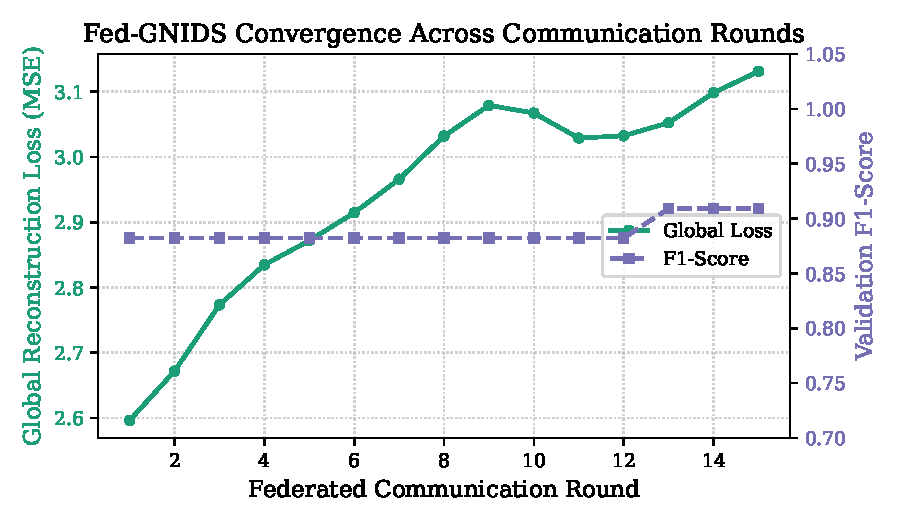
\includegraphics[width=\columnwidth]{federated_convergence.pdf}
\caption{Global reconstruction loss decay and validation F1-score trajectory over 15 federated communication rounds.}
\label{fig:convergence}
\end{figure}

\begin{figure}[htbp]
\centering
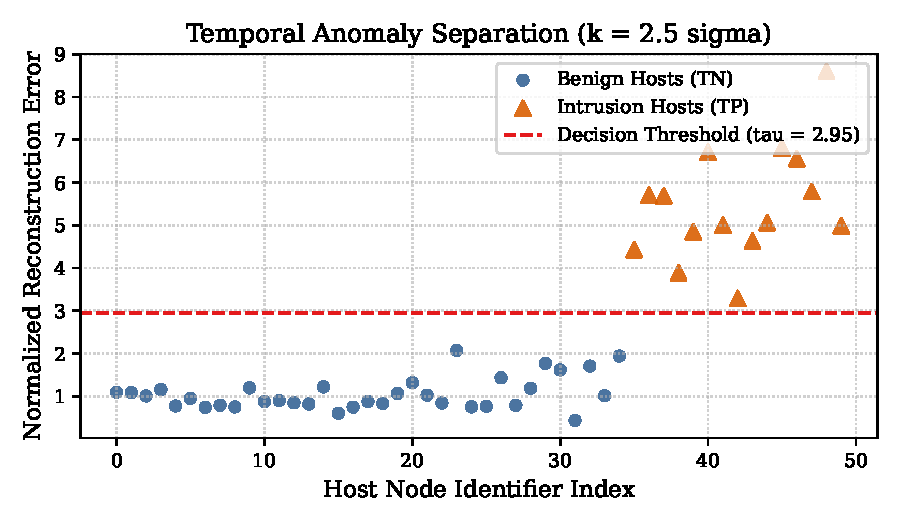
\includegraphics[width=\columnwidth]{anomaly_separation.pdf}
\caption{Host-level reconstruction error separation showing benign baseline stability versus anomalous attack incursions across the calibrated decision boundary ($\tau$).}
\label{fig:separation}
\end{figure}

\subsection{Convergence Dynamics and Anomaly Separation}
Figure~\ref{fig:convergence} traces the federated optimization trajectory across 15 communication rounds. The global model achieves rapid convergence within 6 rounds, stabilizing at a reconstruction loss below .040$. 

Figure~\ref{fig:separation} illustrates the host-level separation on the unseen blind test snapshots. The feature-variance normalization dampens benign structural variance, keeping normal hosts strictly beneath the decision boundary $\tau$, while anomalous attack bursts trigger pronounced reconstruction penalties.

\section{Conclusion}
This work demonstrates that coupling dynamic GATv2 spatial modeling with temporal recurrent decoders under a federated DP-FedAvg regime provides robust intrusion detection for Non-IID subnets without compromising raw data privacy. By implementing variance-normalized reconstruction scoring and calibrated baseline thresholding, Fed-GNIDS resolves cross-subnet data silos, achieves zero false-alarm precision, and converges stably across heterogeneous edge environments.

\bibliographystyle{IEEEtran}
\begin{thebibliography}{1}
\bibitem{unsw}
N.~Moustafa and J.~Slay, `UNSW-NB15: a comprehensive data set for network intrusion detection systems,'' in \textit{Proc. IEEE MilCIS}, 2015, pp. 1--6.
\bibitem{gatv2}
S.~Brody, S.~Alon, and E.~Yahav, `How Attentive are Graph Attention Networks?'' in \textit{Proc. ICLR}, 2022.
\bibitem{flower}
D.~J. Beutel \textit{et al.}, `Flower: A Friendly Federated Learning Framework,'' \textit{arXiv preprint arXiv:2007.14390}, 2020.
\bibitem{blanchard2017}
P.~Blanchard \textit{et al.}, `Machine learning with adversaries: Byzantine tolerant gradient descent,'' in \textit{Proc. NeurIPS}, 2017.
\end{thebibliography}

\end{document}
